\section{Overview}


This tutorial demonstrates how to diagnose the performance of MCMC simulations, such as the output from \RevBayes.
You will create a phylogenetic model for the evolution of DNA sequences under a JC, HKY85, GTR, GTR+Gamma and GTR+Gamma+I substitution model.
For all these models you will perform an MCMC run to estimate phylogeny and other model parameters.

\subsection*{Requirements}
We assume that you have completed the following tutorials:
\begin{itemize}
\item RB\_MCMC\_Tutorial
\end{itemize}



\newpage
\FloatBarrier
\section{Exercise: Assessing Performance of MCMC Simulations}

``{\it You can never be absolutely certain that the MCMC is reliable, you can only identify when something has gone wrong.}'' Andrew Gelman

\bigskip
Model-based inference is, after all, based on the model.
Careful research means being vigilant both regarding the choice of model and rigorously assessing our ability to estimate under the chosen model. 
The first issue---model specification, which actually entails three closely related issues---is critically important for the simple reason that unbiased estimates can only be obtained under a model that provides a reasonable description of the process that gave rise to our data. 
{\it Model selection} entails assessing the {\it relative fit} of our dataset to a pool of candidate models. 
Rankings are based on model-selection methods that compare the relative fit of candidate modes based either on their maximum-likelihood estimates (which measures the fit of the data to the model at a single point in parameter space), or on marginal likelihood of the candidate models (which measures the average fit of the candidate models to the data). 
{\it Model adequacy}---an equally important but relatively neglected issue---assesses the absolute fit of the data to the model. 
{\it Model uncertainty} is related to the common (and commonly ignored) scenario when multiple candidate models provide a similar fit to the data: in this scenario, conditioning on {\it any single} model (even the best) will lead to biased estimates, and so model averaging is required to accommodate uncertainty in the choice of model.

Much less concern is given to the second aspect of model-based inference: the ability to obtain reliable estimates under the chosen model(s). 
The implicit assumption, it seems, is that if a model is implemented correctly, and if that implementation is  successfully used to obtain an estimate from a given dataset, then we must have performed valid inference under the model. 
This would be perfectly sound reasoning if inferences were based on analytical methods. 
Owing to the complexity of the models, however, it is not possible to estimate phylogenetic parameters analytically.
Instead, parameter estimates are based on numerical methods. In the case of maximum-likelihood estimation, these are typically hill-climbing algorithms that attempt to search the profile likelihood to identify the vector of point estimates of all phylogenetic model parameters that jointly maximize the likelihood of observing the data under the model. 
The reliability of these algorithms can (and should) be assessed by comparing estimates obtained from repeated analyses that are initiated from random points in parameter space. 
Because there is only one {\it maximum} likelihood estimate, the terminal values estimated by replicate runs should be identical (within the precision of computer memory).

In the Bayesian statistical framework, inferences focus on the joint posterior probability density of phylogenetic model parameters, which is approximated by Markov chain Monte Carlo (MCMC) algorithms. 
It may be comforting to know that, in theory, an {\it appropriately constructed} and {\it adequately run} MCMC simulation is guaranteed to provide an arbitrarily precise description of the joint posterior probability density. 
In practice, however, even a given MCMC algorithm that provides reliable estimates in {\it most} cases will nevertheless fail in {\it some} cases and is not guaranteed to work for any given dataset. 
This raises an obvious question: ``When do we know that an MCMC algorithm provides reliable estimates for a given empirical analyses''. The answer is simple: \emph{Never}.
%[Leaving aside, for the moment, questions regarding the definitions of an {\it appropriately constructed} and {\it adequately run} chain.] 

Fortunately, this problem is not unique to the field of phylogenetics. 
Much of Bayesian inference outside our field also relies on MCMC algorithms to approximate the joint posterior probability density of parameters: similar concerns regarding the reliability of those inferences has motivated the development of a suite of diagnostic tools to assess MCMC performance. 
The trick is learning how to use these tools effectively and rigorously, especially for analyses that entail complex phylogenetic models and/or large datasets.

\bigskip
\subsection{MCMC Basics}

The ability to rigorously diagnose MCMC performance requires familiarity with some basic concepts from probability theory (discussed last time) and a strong intuitive understanding of the underlying mechanics---we need to know how the algorithms work in order to understand when they are not working. 
In this installment we'll briefly cover the mechanics of the Metropolis Hastings MCMC algorithm.

Recall that Bayesian inference is focused on the posterior probability density of parameters.
The posterior probability of the parameters can, in principle, be solved using Bayes' theorem.
However, (most) phylogenetic problems cannot be solved analytically, owing mainly to the denominator of Bayes' theorem---the marginal likelihood requires solving multiple integrals (for all of the continuous parameters, such as branch lengths, substitution rates, stationary frequencies, etc.) for each tree, and summing over all trees.

Accordingly, Bayesian inference of phylogeny typically resorts to numerical methods that approximate the posterior probability density. 
There are many flavors of Markov chain Monte Carlo (MCMC) algorithms---Gibbs samplers, Metropolis-coupled and reversible-jump MCMC, etc.---we will consider the Metropolis Hastings (MH) algorithm because it is commonly used for phylogenetic problems, and because it is similar to many other variants (which we will cover elsewhere). 
Note that MCMC and Bayesian inference are distinct animals: they have a relationship similar to that between 'optimization algorithms' and ‘maximum-likelihood estimation.' 
Some Bayesian inference can be accomplished without MCMC algorithms, and MCMC algorithms can be used to solve problems in non-Bayesian statistical frameworks.

To introduce the MH algorithm, we will imagine a robot that is programed to explore an area. 
Specifically, the goal of our robot is to generate a topographic map of an unknown terrain. 
This terrain has a total surface area of one hectare. 
We deploy our robot by parachute at a random location within the terrain. 
We have programmed the robot with three simple rules:

\begin{enumerate}
\item{If a proposed step will take the robot uphill, it automatically takes the proposed step.}

\item{If a proposed step will take the robot downhill, it divides the elevation of the proposed location by the elevation of the current location: we call this quotient $R$. 
It then generates a uniform random number, $U[0,1]$. 
If $U<R$, the robot takes the proposed step; otherwise, it stays put.}

\item{The distribution for proposing steps is symmetrical. 
That is, the probability of proposing a step (but not necessarily accepting a proposed step) from point A to point B is equal to the probability of proposing a step from point B to point A.}
\end{enumerate}

We allow our little robot to wander through the terrain following these three simple rules. 
At prescribed intervals  ({\it e.g.}, every $10$ proposed steps), the robot records the details of his position (his elevation, latitude, longitude, etc.) in a log. 
If we allow our robot to wander long enough, his log is guaranteed to provide an arbitrarily precise description of the topography of the terrain. 

Let's consider a slightly more formal description of the Metropolis-Hastings MCMC algorithm. 
First some preliminaries. 
This algorithm entails simulating a Markov chain that has a stationary distribution that is the joint posterior probability density of phylogenetic model parameters. 
The `state' of the chain is a set of parameter values that fully specify phylogenetic model: {\it e.g.}, a tree topology, a vector of branch lengths, and a set of parameters specifying the stochastic model of trait change ({\it e.g.}, for the GTR + $\Gamma$ substitution model, this comprises a vector of values for the four stationary frequencies, a vector of values for the six exchangeability parameters, and the value of the alpha parameter describing the shape of the gamma-distributed among-site rate variation). 
Under the robot analogy, the state of the chain corresponds to a unique point in the terrain. 
The Markov property of the MCMC reflects the fact that the next state of the chain only depends on the current state of the chain, but not on previous states---that is, the past affects the future only through the present. 
The Monte Carlo aspect of the MCMC reflects the fact that it is a simulation: it is a numerical method that relies on repeated random sampling.

Now, on to the MH algorithm:

\begin{enumerate}
\item{Initialize the chain with values for all parameters, including the tree topology, $\tau$, the vector of branch lengths $\nu$, and substitution model parameters $\pi_i$, $q_i$, $\alpha$. 
We will call the set of model parameters $\theta$. The initial parameter values might be specified arbitrarily, or might be drawn from the corresponding prior probability density for each parameter.}

\item{Select a single parameter (or set of parameters) to alter according to its proposal probability. 
%For example, here are the default proposal probabilities used by \MrBayes:
%
%
%We can see that $\sim 1\%$ of the time ({\it i.e.}, with probability $\sim 0.01$), the MCMC will propose changes to the exchangeability (`revmat') and stationary frequency (`pi') parameters using a `Dirichlet' proposal mechanism, and an equal effort proposing changes to the same parameters using something called a `Slider' proposal mechanism.
%Conversely, $\sim 10\%$ of the time ({\it i.e.}, with probability $\sim 0.1$), the MCMC will propose changes to the tree and branch lengths (`Tau and V') using the `extending SPR' proposal mechanism, and with equal probability using the `extending TBR', `extending NNI' and the `parsimony SPR' proposal mechanisms.

For the moment, we won't worry about the details of these proposal mechanisms---they basically involve different ways of `poking' the current parameter value, $\theta$, to generate a new (proposed) parameter value, $\theta ^{\prime}$. 
The important question at the moment is: Where do these proposal probabilities come from? 
The answer is: experience. 
We want to design the MCMC such that it invests effort in a given parameter in proportion to the difficulty of approximating that parameter. 
Note that the MCMC summarized above will spend $\sim 2\%$ of its time proposing changes to the exchangeability and stationary frequency parameters, but will invest $\sim 40\%$ of its time proposing changes to the topology parameter. 
Experience suggests that the tree topology is a more difficult parameter for the MCMC to approximate relative to the exchangeability and stationary frequency parameters (in fact, it appears that the developers of \verb!MrBayes! determined from their experience that the topology is $\sim 20$ times harder to approximate).}

\item{Propose a change to the selected parameter using the parameter-specific proposal
mechanism. 
Different parameters may naturally have different prior probability densities---for example, the stationary frequencies are proportions (ranging between $0$ and $1$), and so are conveniently described using a Dirichlet prior probability density, whereas the alpha-shape parameter can range between zero and infinity, so is better described using a uniform prior probability density. 
Different kinds of prior probability densities will have specific proposal mechanisms---for example, there is something called a `Dirichlet' proposal mechanism that is used to propose new values for parameters described by a Dirichlet prior, and something called a `Slider' proposal mechanism that is used to propose new values for parameters described by a uniform prior. 
(Again, we'll go into the gory details of these proposal mechanisms another time. 
The main idea for now is that the proposal mechanisms generate a new parameter value by poking the current parameter value.)

The design of proposal mechanisms is something of a dark art---trial and error are used to guide the development of mechanisms that work well. 
Nevertheless, there are basic criteria that the proposal mechanisms must meet. 
All proposal mechanisms must be:

%\begin{enumerate}
\begin{enumerate}
\item{stochastic (new parameter values must be proposed `randomly')}

\item{irreducible (all parameter values must be potentially accessible by the chain)}

\item{aperiodic (the proposal mechanism must not induce epicycles of the chain)}
%\end{enumerate}
\end{enumerate}}

\item{Calculate the probability of accepting the proposed change, $R$:

\begin{align}
R = \text{min}\Bigg[1, \underbrace{\frac{P(X \mid \theta ^{\prime})}{P(X \mid \theta )}}_{\text{likelihood ratio}} \cdot \underbrace{\frac{ P(\theta ^{\prime})}{P(\theta)}}_\text{prior ratio} \cdot \underbrace{\frac{P(\theta \mid \theta ^{\prime})}{P(\theta ^{\prime} \mid \theta)}}_\text{proposal ratio} \Bigg]
\end{align}

The acceptance probability, $R$, is either equal to one or the product of three ratios' so long as that product is less than one (because $R$ is a probability, so it cannot be greater than one). 
So, what are these three ratios?

\textbf{Likelihood ratio:} the likelihood ratio is simply the likelihood of the observations given the proposed value of the parameter, divided by the likelihood of the observations given the current value of the parameter. 
We can calculate the likelihood for any given parameterization of the phylogenetic model using the pruning (Felsenstein) algorithm.

\textbf{Prior ratio:} in Bayesian inference, each parameter is a random variable, and so is described by a prior probability density. 
Accordingly, we can `look up' (calculate) the prior probability of any specific parameter value. 
The prior ratio is simply the prior probability of the proposed and current parameter values.

\textbf{Proposal ratio:} the proposal ratio is the probability of proposing the current parameter value given the proposed parameter value, divided by the converse. 
This is also called the Hastings ratio. 
This is equivalent to the rule that forces our robot to propose steps symmetrically; {\it i.e.}, that the probability of proposing a step from point A to point B in the terrain is equal to the probability of proposing a step from point B to point A. 
For inference problems in which the dimensions of the model are static, the proposal ratio is usually equal to one (we'll discuss exceptions to this in the context of reversible-jump MCMC in a future post).

Note that if the proposal ratio is equal to one, the acceptance probability, $R$ is based only on the product of the likelihood and prior ratios. Does that ring a bell? 
[Hint: think of Bayes' theorem.] 
[Hint 2: think of the right side of Bayes' theorem.] 
[Hint 3: think of the numerator of the right side of Bayes' theorem.] 
That is, the posterior probability is proportional to the product of the likelihood and prior probability. 
Accordingly, the acceptance probability is the posterior probability of the proposed state divided by the posterior probability of the current state. 
Just as we programmed our robot, if the ratio of the proposed and current elevations (posterior probabilities) is greater than 1 ({\it i.e.}, it is an uphill step), we always accept the proposed change. 
When the ratio of the proposed and current elevations is less than 1 ({\it i.e.}, it is an downhill step), we may or may not take the proposed step (stay tuned).}


\item{Generate a uniform random number between zero and one, $U[0,1]$. If $U<R$, accept
the proposed change; otherwise, the current state of the chain becomes the next state of the chain. 
Downhill moves will be accepted `randomly' in proportion to the difference in elevation.}

\item{Repeat steps $2-5$ an `adequate' number of times.}
\end{enumerate}

\textbf{That's it!} Notice that the decision to accept or reject proposed steps in the MCMC (and thus to sample from the joint posterior probability density) is based exclusively on the likelihood and prior probability of the proposed and current states---two quantities that are easy to calculate. 
The beautiful, fantabulous achievement of the Metropolis-Hastings algorithm is the slaying of the beastly denominator of Bayes' theorem. 
Specifically, the algorithm allows us to do inference while entirely avoiding the need to calculate the (completely intractable) marginal likelihood!

Approximating the joint posterior probability density is based on samples from the MCMC: a chain following the simple rules outlined above will sample parameter values in proportion to their posterior probability. 
That is, the proportion of time that the chain spends in any particular state is a valid approximation of the posterior probability of that state ({\it e.g.}, if a clade is present in $87\%$ of the samples drawn from the chain, then the posterior probability of that clade is estimated to be $0.87$).

Why do we accept proposals to states with lower posterior probability? 
People familiar with maximum-likelihood estimation often misunderstand the purpose of accepting proposals to states with a lower posterior probability. 
In maximum-likelihood inference, the game is to simply climb relentlessly and mindlessly up the likelihood surface in search of the very tip of the globally highest peak. 
Accordingly, the only reason these zombie hill climbers might consider a downward move would be motivated by concerns that they were currently climbing up a local (rather than global) optimum. 
By contrast, Bayesians are not just interested in the elevation of the very tip of the absolute peak of the posterior probability surface, but rather are interested in exploring and estimating the entire joint posterior probability density---we want topographical map of the entire posterior probability, not the elevation of the tip of the very highest peak in parameter space.

This survey of the joint posterior probability density results in a more robust inference procedure (inferences are averaged over the joint posterior probability of all model parameters), and allows us to estimate and evaluate the marginal posterior probability density for each of the parameters (these can be viewed by querying the MCMC samples with respect to the parameter of interest---we will do this in future tutorials). 
Accordingly, it is not sufficient for the chain to reach the peak of the joint posterior probability density; we need the chain to mix over the entire stationary distribution, spending time at each location in proportion to its posterior probability.

Next to the specification of priors (which are inspired by much more philosophical considerations), performance of the MCMC algorithm used to approximate the joint posterior probability distribution is the greatest concern associated with Bayesian inference (it is certainly a more general concern, as it holds even when the priors are uncontroversial, and, in my opinion, is a more legitimate and practical concern). 
There are three closely related issues associated with MCMC performance: (1) convergence (is the robot sampling from the stationary distribution); (2) mixing (is the robot efficiently moving over the posterior probability density); and (3) adequacy (has the robot collected sufficient samples from the target distribution to describe it adequately).


\bigskip
\section{Diagnosing MCMC performance}

\subsection{Running Markov chain Monte Carlo Simulations \& Assessing Output}\label{secUnif} 


\subsubsection{Data \& Model}

We provide the data file(s) which we will use in this tutorial.
You may want to use your own data instead.
In the \cl{data} folder, you will find the following files
\begin{itemize}
\item
\cl{primates\_and\_galeopterus\_cytb.nex}: Alignment of the \textit{cytochrome b} subunit from 23 primates representing 14 of the 16 families (\textit{Indriidae} and \textit{Callitrichidae} are missing). Note that there is one outgroup species included: \emph{Galeopterus variegatus}.
\end{itemize}
This is the same data and model as we used previously in the CTMC tutorial.

Look at Model file \& MCMC file in a text editor.


\subsubsection{Running MCMC}

Let us now explore the behavior of our Markov chain.
The aim here in these exercises is to visually inspect the output generated by \RevBayes.
You should look at the trace plots using \verb!Tracer!.
Watch out for badly mixing chains, poor performance of the MCMC and correlated parameter estimates.


The first analysis which we perform is specified as follows:
\begin{itemize}
\item{uniform GTR+I+G}
\item{single move per cycle}
\item{large proposal for all parameters}
\item{no-pre-burnin}
\end{itemize}
You can run this analysis directly using
{\tt \begin{snugshade*}
\begin{lstlisting}
source("scripts/mcmc_run1.Rev")
\end{lstlisting}
\end{snugshade*}}
The operator summary provides you with an overview of the moves that you have used for this MCMC run.
It tells you what the weight for each move was, the variables it has been working on, the number of times the move was used, and how often the move was accepted.
Good acceptance rates for continuous parameters are between 20\% and 60\%.
For discrete characters, such as the phylogeny, there is no rule of thumb what good acceptance is.
Instead, the acceptance rate of tree topology proposal strongly depends on the current data.

Now let us open the generated output file in \verb!Tracer!.
The file should be called output/primates\_cytb\_test1.log.

What you may notice is that the ESS are very low and the MCMC is mixing very poor.
This is not good. 
We'll try a new analysis but instead run multiple moves per iteration.
The new setting is:
\begin{itemize}
\item{uniform GTR+I+G}
\item{\it multiple moves per cycle}
\item{large proposal for all parameters}
\item{flat \& low proposal weights}
\item{no-pre-burnin}
\end{itemize}
We achieve this by setting \cl{moveschedule="random"} (which is the default) as an argument for the MCMC algorithm.
You can run this analysis in \RevBayes using
{\tt \begin{snugshade*}
\begin{lstlisting}
source("scripts/mcmc_run2.Rev")
\end{lstlisting}
\end{snugshade*}}
Look at the output in \verb!Tracer! again.
You should see that the ESS values are still very low and the chain is still not mixing well.

One issue that you see is that shape and rate parameter \cl{alpha} for the among-site-rate-variation is updated not often enough.
It is quite likely that our move proposed too many bad new parameters.
So let us change the window size for the scaling move applied on \cl{alpha} from
{\tt \begin{snugshade*}
\begin{lstlisting}
moves[++mvi] = mvScale(alpha, lambda=50.0, weight=2.0)
\end{lstlisting}
\end{snugshade*}}
to
{\tt \begin{snugshade*}
\begin{lstlisting}
moves[++mvi] = mvScale(alpha, lambda=1.0, weight=2.0)
\end{lstlisting}
\end{snugshade*}}
This will give us now the following set-up:
\begin{itemize}
\item{uniform GTR+I+G}
\item{multiple moves per cycle}
\item{\it smaller proposals for \cl{alpha}}
\item{flat \& low proposal weights}
\item{no-pre-burnin}
\end{itemize}
Run the analysis file and look how often the scaling Move is now accepted.
{\tt \begin{snugshade*}
\begin{lstlisting}
source("scripts/mcmc_run3.Rev")
\end{lstlisting}
\end{snugshade*}}
Open the output and look at it in \verb!Tracer!.
We are now getting better ESS values and better mixing of the MCMC.

That worked quite well but it seems to be cumbersome to adjust all the tuning parameters of the moves manually.
Instead, let us allow \RevBayes to auto-tune the moves.
Just change \cl{tune=true} for all moves where it was \cl{tune=false} before.
Now, also include a pre-burnin.
The pre-burnin runs if you say \cl{mymcmc.burnin(generations=1000,tuningInterval=100)}.
This runs a chain for 1000 iterations and updates the tuning parameters, such as the window size, so that you achieve a good acceptance rate.
That means, if previously a move accepted too few proposal it will decrease the window size.

Here is the new model set-up:
\begin{itemize}
\item{uniform GTR+I+G}
\item{multiple moves per cycle}
\item{flat \& low proposal weights}
\item{\it pre-burnin (with scale adjusted from previous)}
\end{itemize}
Run the analysis in \RevBayes:
{\tt \begin{snugshade*}
\begin{lstlisting}
source("scripts/mcmc_run4.Rev")
\end{lstlisting}
\end{snugshade*}}
Look at the output given by the operator summary.
Notice how the tuning parameters have been updated.
Also look at the output in \verb!Tracer!.
You will see that the ESS values are much better because the chain is mixing better.

%In the next step we chain the proposal weights so that moves are used more often, especially for the parameters that are not mixing well.
%Our new setting is:
%\begin{itemize}
%\item{uniform GTR+I+G}
%\item{multiple moves per cycle}
%\item{\it variable proposal weights}
%\item{pre-burnin (with scale adjusted from previous)}
%\end{itemize}
%Run the \RevBayes~analysis.
%{\tt \begin{snugshade*}
%\begin{lstlisting}
%source("scripts/analysis/mcmc_run5_PS0.Rev")
%mymcmc.operatorSummary()
%\end{lstlisting}
%\end{snugshade*}}
%When you look at the output you will see that it now mixing fairly well.
%So let us focus on the approximated posterior distribution.
%Specifically, what is the posterior mean of the tree-length (\cl{TL})?
%This tree-length is surprisingly large. 
%We could specify a prior distribution with a lower expectation (mean) on the tree-length.
%\begin{itemize}
%\item{uniform GTR+I+G}
%\item{multiple moves per cycle}
%\item{variable proposal weights}
%\item{pre-burnin (with scale adjusted from previous)}
%\item{\it branch length prior to \cl{dnExponential(20.0)} (mean 0.05)}
%\end{itemize}
%Run the new analysis in \RevBayes.
%{\tt \begin{snugshade*}
%\begin{lstlisting}
%source("RevBayes_scripts/analysis/mcmc_run6_PS0.Rev")
%mymcmc.operatorSummary()
%\end{lstlisting}
%\end{snugshade*}}
%If you look at the results from this analysis, you will notice that the tree-length estimates are better.
%However, if you look at the joint posterior density of the tree-length (\cl{TL}) and the probability of a site being invariant (\cl{pinvar}), then you will notice that there is a very high correlation between these two.
%It seems as if our model is over-parameterized.
%To resolve this issue we need to remove/fix some of our parameters.
%Open the data file and look how variable each site is. What is your impression on how many sites are invariant?
%
%We remove the gamma distributed rate variation among sites because most sites either seem to be fixed or evolve under our GTR model.
%We also reset the branch length priors to \cl{dnExponential(10.0)}.
%\begin{itemize}
%\item{uniform GTR+I}
%\item{multiple moves per cycle}
%\item{variable proposal weights}
%\item{pre-burnin (with scale adjusted from previous)}
%\end{itemize}
%Run the new script in \RevBayes.
%{\tt \begin{snugshade*}
%\begin{lstlisting}
%source("RevBayes_scripts/analysis/mcmc_run7_PS0.Rev")
%mymcmc.operatorSummary()
%\end{lstlisting}
%\end{snugshade*}}
%Look again at output in \verb!Tracer!.
%We seem to be doing a pretty good job with one chain.
%This is our visual method to inspect the MCMC output. 

\subsection{Comparing your output to the prior}
Next, let's compare it to the prior.
Here we want to see how much information we actually have from the data and how much our prior influenced our posterior estimates.
Run now an analysis that does not use the data.
You can do this in \RevBayes the exact same way as running an MCMC on the exact same model, you only need to call \cl{mymcmc.run(1000,underPrior=true)}.
{\tt \begin{snugshade*}
\begin{lstlisting}
source("scripts/mcmc_run_prior.Rev")
\end{lstlisting}
\end{snugshade*}}
Load both the MCMC output under the prior and the posterior into \verb!Tracer!.
Compare the approximated distributions on each parameter between both outputs.



Apply multiple-run diagnostics:
\begin{itemize}
\item{PSRF}
\item{ASDSF}
\item{comparetrees}
\end{itemize}

	
	

\bigskip
\section{Semi-automatic MCMC diagnosis using bonsai}

\definecolor{shadecolor}{RGB}{183,107,137}
Diagnosing MCMC performance manually can be extremely cumbersome, especially for more complex models.
The R package bonsai performs a standard set of diagnostics on MCMC output and generates a report that highlights potentially pathological MCMC behaviors.
To use bonsai, download the package source from \href{https://github.com/mikeryanmay/bonsai}{https://github.com/mikeryanmay/bonsai}, launch the R console, and install the package from source by following the instructions on the bonsai main page (making sure to install the packages that bonsai relies on as well):
{\tt \begin{snugshade*}
\begin{lstlisting}
install.packages(packages=c('coda','tools','RColorBrewer','entropy','xtable'),dependencies=TRUE)
install.packages('< path to bonsai >',repos=NULL,type='source')
library(bonsai)
\end{lstlisting}
\end{snugshade*}}

Move the output files from \texttt{run7} to the folder \verb!.../RB_MCMC_Tutorial/output/output_for_bonsai!.

Going back to the R console, provide a name for the project.
{\tt \begin{snugshade*}
\begin{lstlisting}
project <- 'Fagus run 7'
\end{lstlisting}
\end{snugshade*}}

Point bonsai at the directory where we placed our log files.
{\tt \begin{snugshade*}
\begin{lstlisting}
path <- '.../RB_MCMC_Tutorial/output/output_for_bonsai'
\end{lstlisting}
\end{snugshade*}}

Finally, we create the bonsai object and execute the \texttt{runBonsai()} function.
It will generate a report that draws your attention to potential issues.
{\tt \begin{snugshade*}
\begin{lstlisting}
fagus_proj <- bonsai(project=project,path=path)
fagus_proj$runBonsai()
\end{lstlisting}
\end{snugshade*}}

Check the flags generated by bonsai (Figure \ref{fig:flags}; your results may differ). 
Many of these flags may be innocuous; it is up to the user to decide whether a particular flag is truly problematic.
For example, a correlation between \texttt{Likelihood} and \texttt{Posterior} is not problematic; however, a significant p-value for Geweke's diagnostic for \texttt{pi[3]} indicates that this parameter has not converged to its stationary distribution.

\begin{figure}[h!]
\begin{center}
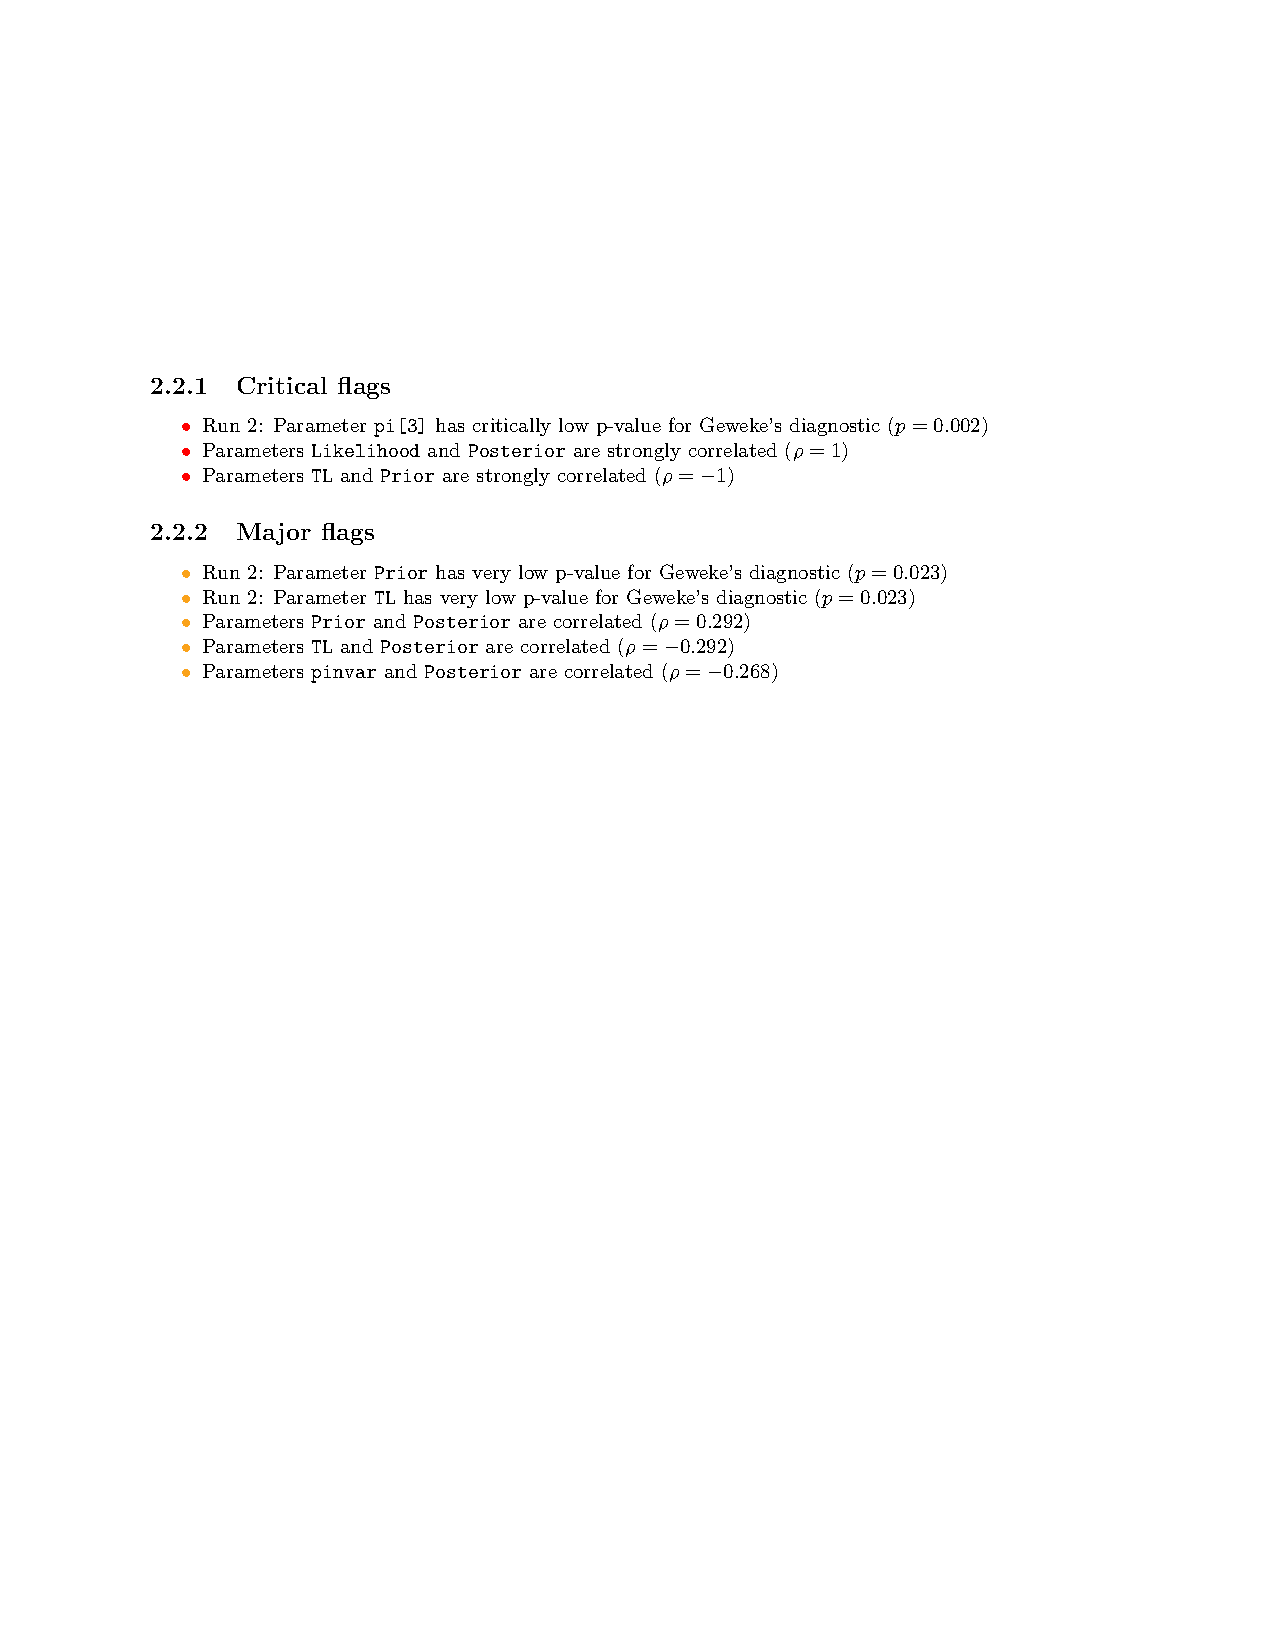
\includegraphics[]{\ResourcePath figures/flags.pdf}
\end{center}
\caption{Flags generated by bonsai.}\label{fig:flags}
\end{figure}

There are additional bonsai reports for more complex models demonstrating a wider array of MCMC pathologies in the \verb!.../RB_MCMC_Tutorial/bonsai_pre_cooked! directory.


\bibliographystyle{sysbio}
\bibliography{\GlobalResourcePath refs}
